\documentclass[twocolumn, a4paper]{article}
\usepackage[a4paper, left = 1.75cm, right = 1.75cm, top = 1.75cm, bottom = 1.75cm]{geometry}
\usepackage[style = numeric, sorting = none]{biblatex}
\usepackage{pgfplots}
\usepackage[T1]{fontenc}
\usepackage{graphicx}
\usepackage[UKenglish]{babel}
\usepackage[UKenglish]{isodate}

\graphicspath{{./images/}}
\addbibresource{refs.bib}

\cleanlookdateon

\renewcommand*{\bibfont}{\footnotesize}

\author{
  George Herbert\\
  \texttt{cj19328@bristol.ac.uk}
}

\title{\vspace{-2em}Optimising and Parallelising d2q9-bgk.c}

\begin{document}

\maketitle

\begin{abstract}
    \texttt{d2q9-bgk.c} implements the Lattice Boltzmann method (LBM) to simulate a fluid density on a lattice.
    This report analyses the techniques I utilised to optimise and parallelise \texttt{d2q9-bgk.c}.
\end{abstract}

\section{Original Code}

I ran the provided \texttt{Makefile} to compile the original \texttt{d2q9-bgk.c}, which executed the GNU Compiler Collection (GCC) (version 4.8.5) with the \texttt{-std=c99} \texttt{-O3} and \texttt{-lm} options.
Table \ref{tab:original} contains the execution time for each test case.

\begin{table}[htbp]
  \begin{center}
  \caption{Execution times of the original code}\label{tab:original}
  \begin{tabular}[t]{l | l} 
      \hline\hline
      Grid Size&Time (s)\\
      \hline
      $128 \times 128$&\texttt{ 29.16}\\
      $128 \times 256$&\texttt{ 58.71}\\
      $256 \times 256$&\texttt{233.32}\\
      $1024 \times 1024$&\texttt{980.89}\\
      \hline
    \end{tabular}
  \end{center}
  \vspace{-1em}
\end{table} 

% I measured the original code to quantify the performance improvements of my latter implementations.
Each time was an average of five runs on a BlueCrystal Phase 4 (BC4) compute node---a Lenovo nx360 M5, which contained two 14-core 2.4 GHz Intel E5-2680 v4 (Broadwell) CPUs and 128 GiB of RAM \cite{bcp4}.
I took an average because of the variation between runs, which existed due to the inconsistent performance of compute nodes.
% Not all compute nodes offer the same performance all of the time, due to differing placement in the data centre, amongst other reasons.

\section{Compiler Optimisations}

% I initially implemented a collection of serial optimisations to improve the performance of \texttt{d2q9-bgk.c}.

\subsection{Intel C Compiler Classic}

I hypothesised that compiling with the Intel C Compiler Classic (ICC) instead of GCC would produce an executable better optimised for BC4's Intel compute nodes.
Table \ref{tab:icc} contains the execution times after compiling with ICC (version 19.1.3.304).
Primarily, the speedup was because ICC vectorized two of the innermost nested loops in the \texttt{collision} procedure, which GCC did not. 

\begin{table}[htbp]
  \begin{center}
  \caption{Execution times using ICC and speedup over the prior implementation}\label{tab:icc}
  \begin{tabular}[t]{l | l l} 
      \hline\hline
      Grid Size&Time (s)&Speedup\\
      \hline
      $128 \times 128$&\texttt{ 22.54}&\texttt{1.29}\\
      $128 \times 256$&\texttt{ 45.56}&\texttt{1.29}\\
      $256 \times 256$&\texttt{179.06}&\texttt{1.30}\\
      $1024 \times 1024$&\texttt{805.21}&\texttt{1.22}\\
      \hline
    \end{tabular}
  \end{center}
  \vspace{-1em}
\end{table}

\subsection{Compiler Options}

I hypothesised that I could compile my program with more aggressive optimisations to improve performance whilst still producing the correct solution.
I compiled my code with the \texttt{-Ofast} option, which implemented additional aggressive floating-point optimisations \cite{icc}.
These aggressive optimisations provided a small performance boost, as evident in Table \ref{tab:compiler_options}.

\begin{table}[htbp]
  \begin{center}
  \caption{Execution times using new ICC options and speedup over the prior implementation}\label{tab:compiler_options}
  \begin{tabular}[t]{l | l l} 
      \hline\hline
      Grid Size&Time (s)&Speedup\\
      \hline
      $128 \times 128$&\texttt{ 22.18}&\texttt{1.02}\\
      $128 \times 256$&\texttt{ 44.42}&\texttt{1.03}\\
      $256 \times 256$&\texttt{176.69}&\texttt{1.01}\\
      $1024 \times 1024$&\texttt{794.44}&\texttt{1.01}\\
      \hline
    \end{tabular}
  \end{center}
  \vspace{-1em}
\end{table}

\section{Serial Optimisations}

I used the Intel Advisor tool to generate a Roofline model, as shown in Figure \ref{fig:roofline_compiler}.

\begin{figure}[htbp]
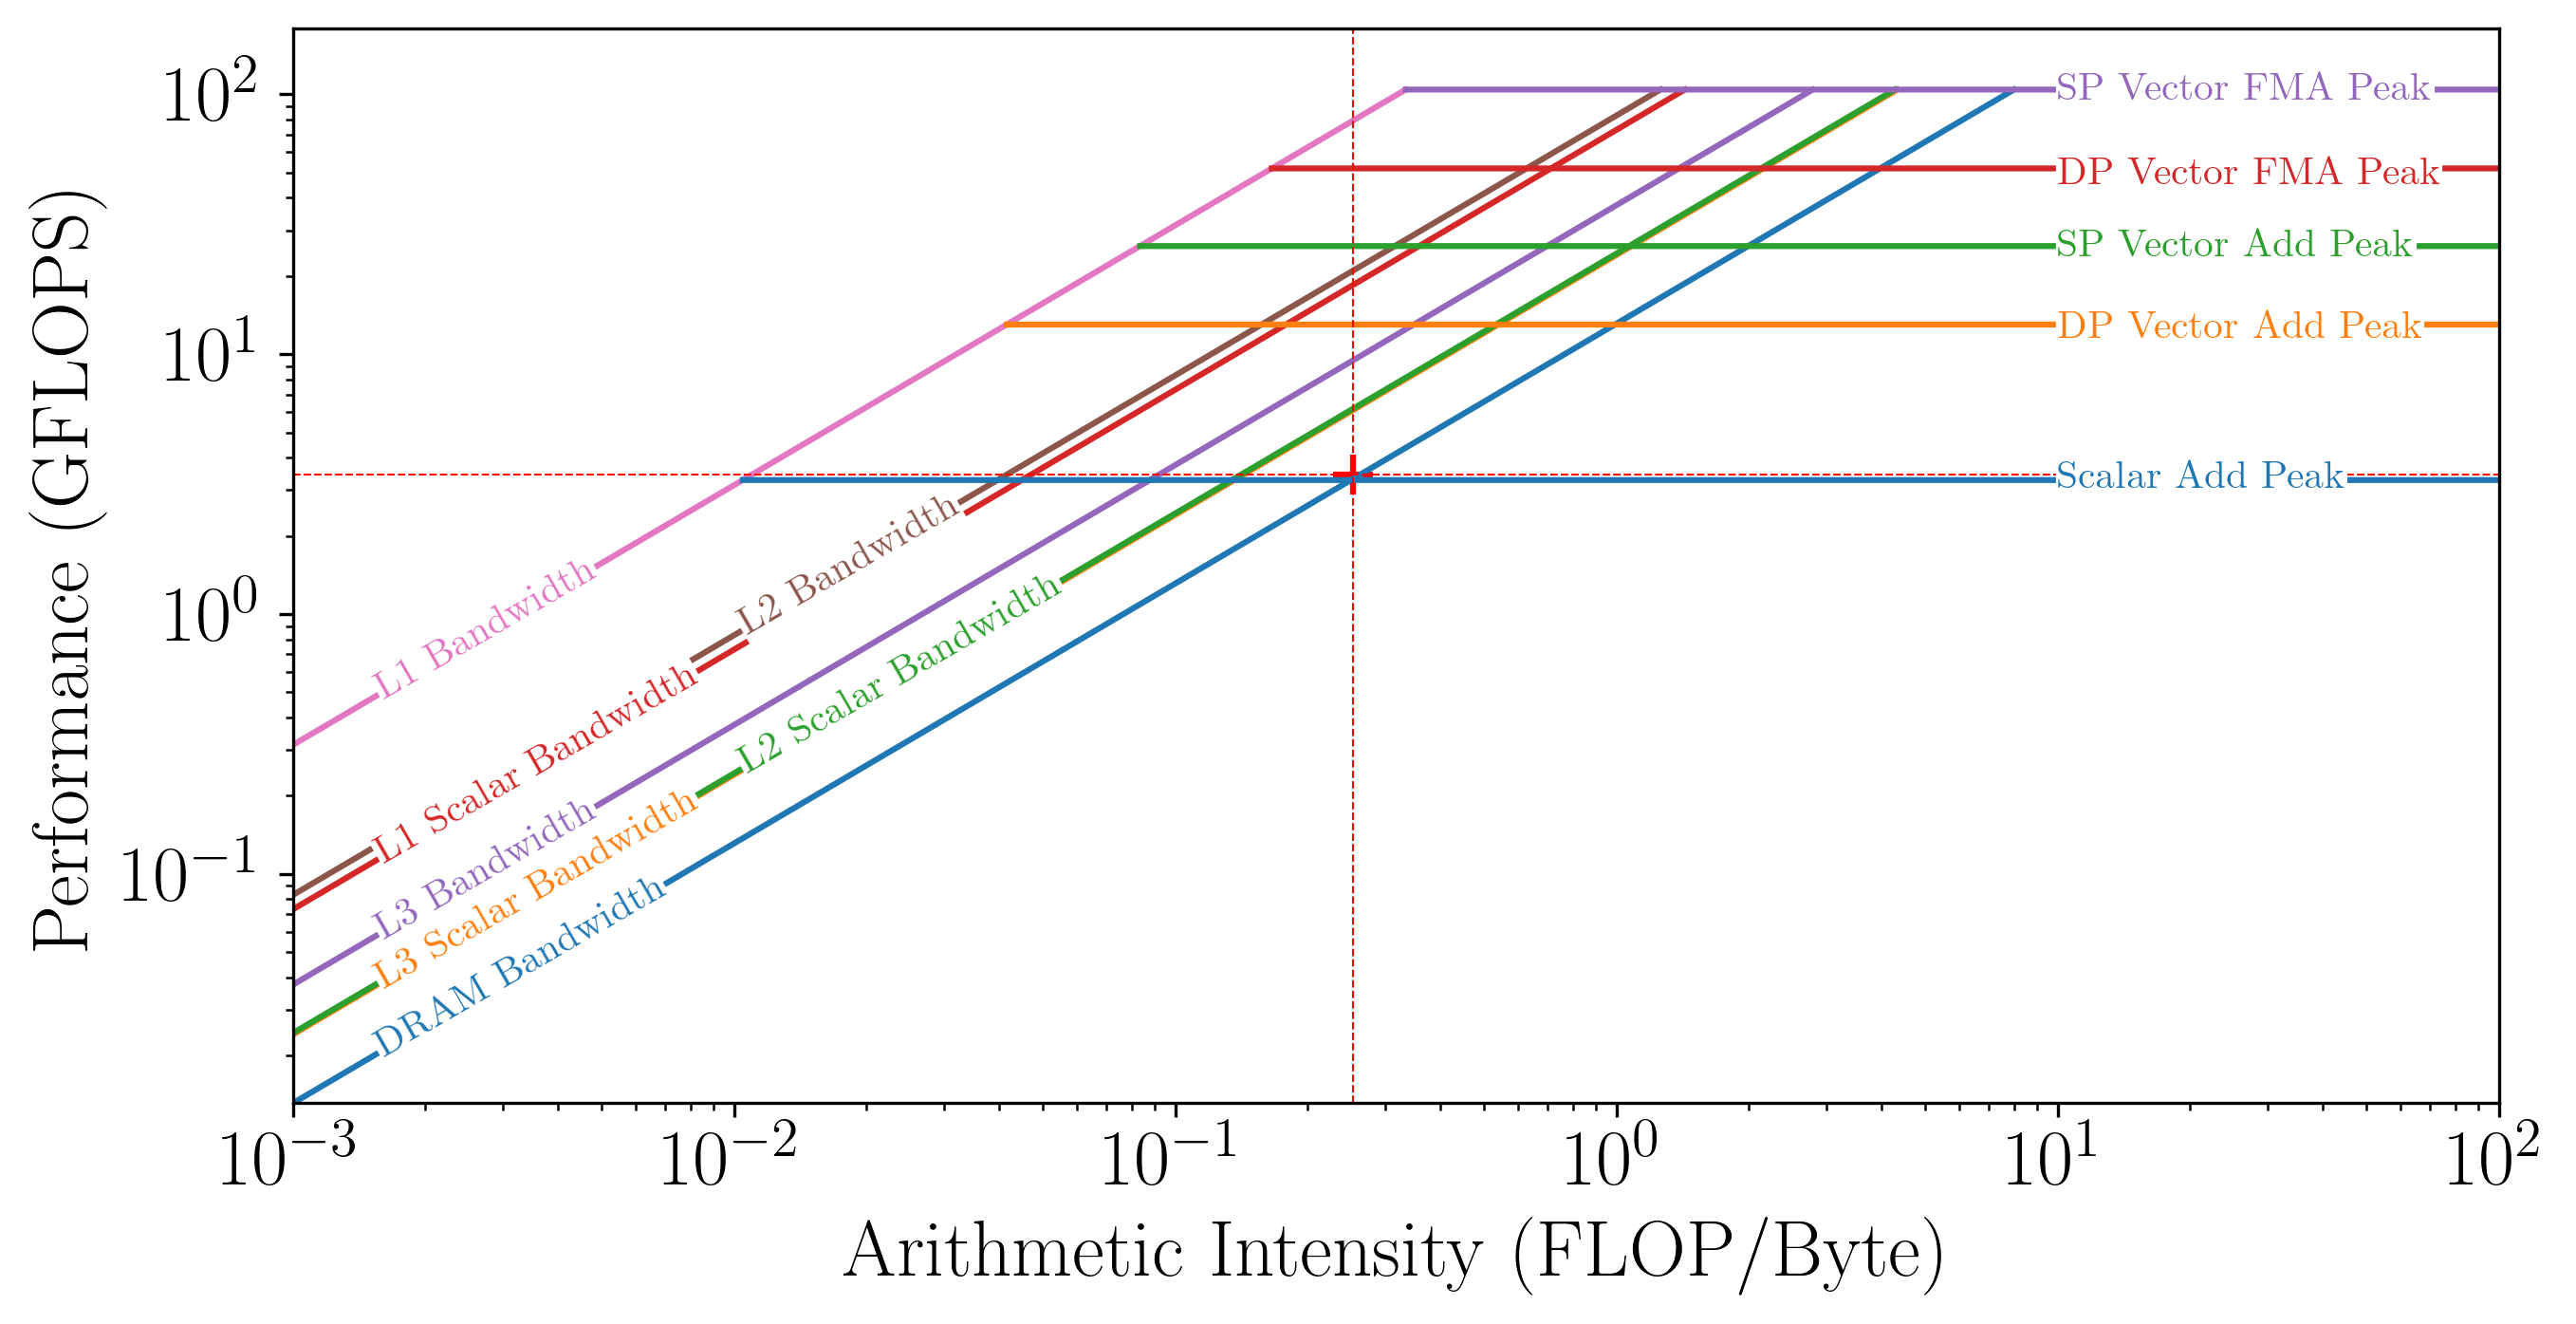
\includegraphics[width=\linewidth]{roofline_compiler.png}
\caption{Roofline model following compilation changes, run on the $1024\times1024$ test case}\label{fig:roofline_compiler}
\end{figure}

I identified several attributes of my program and several key areas to focus my serial optimisations.
For larger grid sizes especially, the LBM implementation in \texttt{d2q9-bgk.c} was a memory bandwidth bound problem.
\texttt{d2q9-bgk.c} achieved an average arithmetic intensity of 0.25 FLOP/byte and performance of 3.44 GFLOPS for the $1024 \times 1024$ test case.

\subsection{Loop Fusion}

Using the Roofline model, I identified that decreasing the number of accesses to memory within each timestep would simultaneously increase my program's performance whilst also increasing the arithmetic intensity, thus raising the performance bound for my latter implementations. 

To accomplish this, I implemented loop fusion.
In the original code, the entire grid was iterated over in four sequential procedures within each timestep: \texttt{propagate}, \texttt{rebound}, \texttt{collision} and \texttt{av\_velocity}.
I fused the four loops within these procedures into a single loop in the \texttt{timestep} function, which enabled me to eliminate the temporary allocations of cell values to the \texttt{tmp\_cells} array.
Instead, my program wrote new values of cells to the \texttt{cells\_new} array; each timestep, my program swapped the pointers of \texttt{cells} and \texttt{cells\_new}.

Table \ref{tab:loop_fusion_pointer_swap} displays the improvements to the execution time.
Moreover, my program's arithmetic intensity increased to 0.29 FLOP/byte, and the performance increased to 3.54 GFLOPS for the $1024 \times 1024$ test case.

\begin{table}[htbp]
  \begin{center}
  \caption{Execution times with loop fusion and pointer swap, and speedup over the prior implementation}\label{tab:loop_fusion_pointer_swap}
  \begin{tabular}[t]{l | l l} 
      \hline\hline
      Grid Size&Time (s)&Speedup\\
      \hline
      $128 \times 128$&\texttt{ 19.42}&\texttt{1.15}\\
      $128 \times 256$&\texttt{ 39.21}&\texttt{1.13}\\
      $256 \times 256$&\texttt{155.64}&\texttt{1.14}\\
      $1024 \times 1024$&\texttt{635.61}&\texttt{1.25}\\
      \hline
    \end{tabular}
  \end{center}
  \vspace{-1em}
\end{table}

\subsection{Arithmetic}

Despite the compiler optimising the arithmetic within each timestep, I hypothesised I could make some manual improvements to reduce my program's execution time further.

Division operations take considerably more time to execute than other basic arithmetic operations, such as multiplication.
I precalculated several values to eliminate unnecessary division operations: \texttt{c\_sq\_r}, the reciprocal of $c^2$; \texttt{two\_c\_sq\_r}, the reciprocal of $2c^2$; and \texttt{two\_c\_sq\_sq\_r}, the reciprocal of $2c^4$, where $c$ was the speed of sound.
I then replaced several division operations with multiplications by these values.

Additionally, I eliminated the repeated calculation of and division by \texttt{tot\_cells} (i.e. the number of cells that were not obstacles) each timestep.
Instead, my program calculated \texttt{tot\_cells} once during the initialisation phase.
It then stored the reciprocal of this value in \texttt{params.num\_non\_obstacles\_r}, which was multiplied with \texttt{tot\_u} to compute each timestep's average velocity.

These arithmetic improvements provided only a slight speedup compared to the previous implementation, as shown in Table \ref{tab:arithmetic_improvements}; this was because memory accesses dominated my program's execution time.
I would expect a more considerable speedup in smaller grid sizes than the test cases provided.

\begin{table}[htbp]
  \begin{center}
  \caption{Execution times with arithmetic improvements and speedup over the prior implementation}\label{tab:arithmetic_improvements}
  \begin{tabular}[t]{l | l l} 
      \hline\hline
      Grid Size&Time (s)&Speedup\\
      \hline
      $128 \times 128$&\texttt{ 19.10}&\texttt{1.02}\\
      $128 \times 256$&\texttt{ 38.49}&\texttt{1.02}\\
      $256 \times 256$&\texttt{153.39}&\texttt{1.01}\\
      $1024 \times 1024$&\texttt{621.52}&\texttt{1.02}\\
      \hline
    \end{tabular}
  \end{center}
  \vspace{-1em}
\end{table}

\section{Vectorization}

Vectorization is the process of converting a scalar implementation to a vector implementation, which enables the compiler to use additional registers to perform single, multiple data (SIMD) operations.

\subsection{Structure of Arrays}

I hypothesised that converting the cells' variables from an array of structures (AoS) to a structure of arrays (SoA) format would suit vectorisation of the inner loop; the SoA format would keep memory accesses contiguous over structure instances.
I altered the \texttt{t\_speed} structure to contain nine pointers, each to an individual array of floats.
Each array of floats contained the values of one vector for each cell within the grid.

The SoA format increased the execution time of my program, as shown in Table \ref{tab:soa}.
Upon inspection, the AoS format had better memory locality in the program's primarily unvectorized form.

\begin{table}[htbp]
  \begin{center}
  \caption{Execution times with SoA and speedup over the prior implementation}\label{tab:soa}
  \begin{tabular}[t]{l | l l} 
      \hline\hline
      Grid Size&Time (s)&Speedup\\
      \hline
      $128 \times 128$&\texttt{ \space19.25}&\texttt{0.99}\\
      $128 \times 256$&\texttt{ \space51.25}&\texttt{0.75}\\
      $256 \times 256$&\texttt{ 211.45}&\texttt{0.73}\\
      $1024 \times 1024$&\texttt{1102.18}&\texttt{0.56}\\
      \hline
    \end{tabular}
  \end{center}
  \vspace{-1em}
\end{table}

\subsection{Memory for Vectorization}

To effect vectorization of the inner loop, I identified that I needed to align the \texttt{cells}, \texttt{cells\_new} and \texttt{obstacles} variables and hint to the compiler that the arrays in the \texttt{t\_speed} structure were not aliased.

Processors efficiently move data located on specific byte boundaries, and compilers can perform optimisations when data access is known to be aligned by 64 bytes \cite{alignment}.
To align the \texttt{cells}, \texttt{cells\_new} and \texttt{obstacles} variables, I replaced calls to the \texttt{malloc} and \texttt{free} procedures with the alignment specific replacements: \texttt{\_mm\_malloc} and \texttt{\_mm\_free}, respectively.
I used the \texttt{\_\_assume\_\_aligned} procedure and  the statement \texttt{\_\_assume(params.nx \% 16 == 0)} to inform the compiler that the dynamically allocated variables were aligned.
Doing so prevented the compiler from generating conservative code, which would have been detrimental to the speed of my implementation.

I compiled my code with the \texttt{-restrict} option and used the \texttt{restrict} keyword to define each of the nine pointers in \texttt{t\_speed}.
The \texttt{restrict} keyword asserted that these pointers were not aliased, which prevented the compiler from performing a runtime check for aliasing.

I implemented the \texttt{\#pragma omp simd} pragma to direct the compiler to utilise SIMD instructions to execute operations within the inner loop in \texttt{timestep}.
I used the \texttt{reduction(+:tot\_u)} clause to ensure the \texttt{tot\_u} variable contained the correct value at the loop's termination.

I compiled with the \texttt{-xAVX2} option to tell the compiler to optimise for Intel processors that support Advanced Vector Extensions 2 (AVX2) (which BC4's compute nodes do) \cite{lenovo}.
I did not compile explicitly with the \texttt{-qopenmp-simd} option since \texttt{-Ofast} enabled it by default \cite{icc}.

Vectorization provided the most considerable improvement of any optimisation that I had implemented to this point, as shown in Table \ref{tab:vectorized}.
The compiler could produce AVX2 instructions that could perform simultaneous operations on up to eight single-precision floating-point numbers.
Furthermore, my implementation achieved an arithmetic intensity of 0.43 FLOP/byte and performance of 10.14 GFLOPS when run on the $1024\times1024$ test case.

\begin{table}[htbp]
  \begin{center}
  \caption{Execution times after vectorizing and speedup over the prior implementation}\label{tab:vectorized}
  \begin{tabular}[t]{l | l l} 
      \hline\hline
      Grid Size&Time (s)&Speedup\\
      \hline
      $128 \times 128$&\texttt{ \space5.77}&\texttt{3.34}\\
      $128 \times 256$&\texttt{ 11.57}&\texttt{4.43}\\
      $256 \times 256$&\texttt{ 41.55}&\texttt{5.09}\\
      $1024 \times 1024$&\texttt{215.52}&\texttt{5.11}\\
      \hline
    \end{tabular}
  \end{center}
  \vspace{-1em}
\end{table}

\section{Parallelism}

% Overall, my serial optimisations (including vectorization) achieved approximately five times speedup over the original implementation.
% However, there was an immense potential for performance improvements by parallelising \texttt{d2q9-bgk.c}. 

\subsection{OpenMP}

Using the Intel Advisor tool, I identified that a large proportion of my program's execution time was in the inner loop in the \texttt{timestep} function.
Therefore, I hypothesised that parallelising the outer loop would substantially improve performance.

OpenMP implements parallelism by launching a set of threads that execute portions of code concurrently.
I included OpenMP's \texttt{\#pragma omp parallel for} pragma, and compiled my code with the \texttt{-qopenmp} option to parallelise the outer loop.
I used the clause \texttt{reduction(+:tot\_u)} to prevent race conditions; the reduction clause informed the compiler to create a copy of the \texttt{tot\_u} variable for each thread (initialised to zero) and to sum the local results at the end of the parallel region.
I used a static schedule to limit the variance between runs.

Table \ref{tab:parallelised} displays the execution times for my parallel implementation when run with 28 threads.
There was a significant speedup over the vectorised implementation because the program could execute iterations of the inner loop in parallel and utilise more cache memory.

\begin{table}[htbp]
  \begin{center}
  \caption{Execution times with 28 threads and speedup over the prior implementation}\label{tab:parallelised}
  \begin{tabular}[t]{l | l l} 
      \hline\hline
      Grid Size&Time (s)&Speedup\\
      \hline
      $128 \times 128$&\texttt{ 1.14}&\texttt{ 5.06}\\
      $128 \times 256$&\texttt{ 1.35}&\texttt{ 8.57}\\
      $256 \times 256$&\texttt{ 3.33}&\texttt{12.48}\\
      $1024 \times 1024$&\texttt{14.38}&\texttt{14.99}\\
      \hline
    \end{tabular}
  \end{center}
  \vspace{-1em}
\end{table}

\subsection{Non-Uniform Memory Access}

Non-uniform memory access (NUMA) is a computer memory design in which memory access time depends on the memory location relative to the processor.
I identified that memory for the \texttt{cells} and \texttt{obstacles} variables was allocated the first thread in my prior implementation, per the first touch policy.
Therefore, I hypothesised that a NUMA-aware implementation would reduce the average memory access time.

I parallelised the initialisation loops for \texttt{cells} and \texttt{obstacles} to ensure that each thread touched the same data in the \texttt{initialise} and \texttt{timestep} procedures.
Additionally, I set the environment variables \texttt{OMP\_PROC\_BIND=true} and \texttt{OMP\_PLACES=cores} to prevent threads from moving cores.

Table \ref{tab:numa} contains the updated execution times for my final NUMA-aware implementation.
The NUMA-aware implementation produced a reasonable performance boost by reducing the average time to access a memory location.

\begin{table}[htbp]
  \begin{center}
  \caption{Execution times with 28 thread NUMA-aware implementation and speedup over both the prior and vectorized implementation}\label{tab:numa}
  \begin{tabular}[t]{l | l  l  l} 
      \hline\hline
      &&\multicolumn{2}{c}{Speedup}\\
      \cline{3-4}
      Grid Size&Time (s)&Prior&Vectorized\\
      \hline
      $128 \times 128$&\texttt{ 0.72}&\texttt{1.58}&\texttt{ 8.01}\\
      $128 \times 256$&\texttt{ 0.80}&\texttt{1.69}&\texttt{14.46}\\
      $256 \times 256$&\texttt{ 2.47}&\texttt{1.35}&\texttt{16.82}\\
      $1024 \times 1024$&\texttt{12.81}&\texttt{1.23}&\texttt{16.83}\\
      \hline
    \end{tabular}
  \end{center}
  \vspace{-1em}
\end{table}

\subsection{Scaling}

I ran my final implementation from 1--28 threads to analyse how my program scaled.
I then calculated the subsequent threads' speedup over a single thread implementation.
Figure \ref{fig:scaling} displays the resultant speedup curves.

\begin{figure}[htpb]
  \centering
  \resizebox{\columnwidth}{!}{
    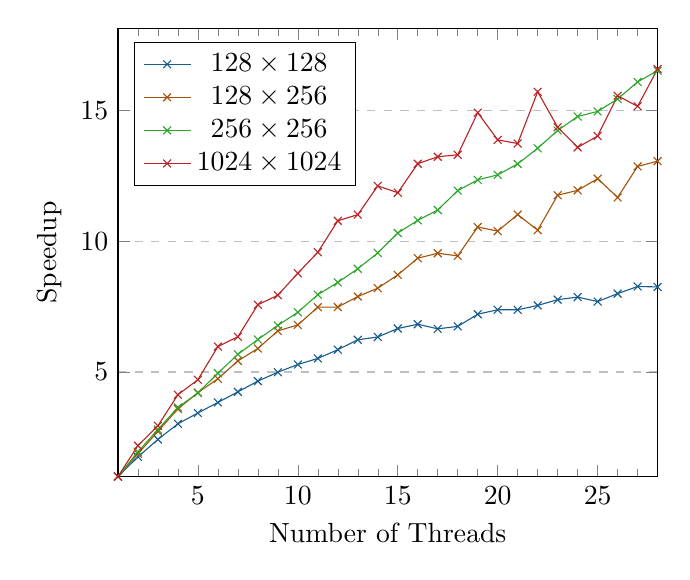
\begin{tikzpicture}
      \begin{axis}[
        xlabel={Number of Threads},
        ylabel={Speedup},
        xmin = 1, xmax = 28,
        ymin = 1,
        % xtick={0, 5, 10, 15, 20, 25},
        % ytick={0,20,40,60,80,100,120},
        legend pos=north west,
        ymajorgrids=true,
        grid style=dashed,
        minor xtick = {1,2,3,4,5,6,7,8,9,10,11,12,13,14,15,16,17,18,19,20,21,22,23,24,25,26,27,28}
      ]
      \addlegendentry{$128\times128$}
      \addplot[color = {rgb:red,31;green,119;blue,180}, mark = x]coordinates{
        (1, 1.0)
        (2, 1.7525169788462858)
        (3, 2.419897249840069)
        (4, 3.0177321760395954)
        (5, 3.4340474353625594)
        (6, 3.8362657949346852)
        (7, 4.241072726461517)
        (8, 4.651864978037027)
        (9, 4.993654422331282)
        (10,5.2882280154084835)
        (11,5.520195387872089)
        (12,5.854579031493787)
        (13,6.23457059163917)
        (14,6.342501046595846)
        (15,6.666023078680611)
        (16,6.829810732132427)
        (17,6.6526516481296065)
        (18,6.746204776109836)
        (19,7.213003419569139)
        (20,7.383978810814603)
        (21,7.383266518002555)
        (22,7.548589923892521)
        (23,7.770076587082373)
        (24,7.86829502746941)
        (25,7.69660960948019)
        (26,8.000150678051229)
        (27,8.274732001825265)
        (28,8.256913368882064)
      };
      \addlegendentry{$128\times256$}
      \addplot[color = {rgb:red,255;green,127;blue,14}, mark = x]coordinates{
        (1, 1)
        (2, 1.87192962)
        (3, 2.728614279)
        (4, 3.588436108)
        (5, 4.211061907)
        (6, 4.74277418)
        (7, 5.426597365)
        (8, 5.901009271)
        (9, 6.574136151)
        (10,6.804566205)
        (11,7.483065988)
        (12,7.486914766)
        (13,7.888917429)
        (14,8.209594871)
        (15,8.719464845)
        (16,9.356809194)
        (17,9.546299879)
        (18,9.445666983)
        (19,10.54931431)
        (20,10.3964243)
        (21,11.02717878)
        (22,10.42891424)
        (23,11.76705845)
        (24,11.95396706)
        (25,12.40123763)
        (26,11.68112555)
        (27,12.86943567)
        (28,13.07066895)
      };
      \addlegendentry{$256\times256$}
      \addplot[color = {rgb:red,44;green,160;blue,44}, mark = x]coordinates{
        (1, 1)
        (2, 1.945477182)
        (3, 2.800216561)
        (4, 3.646333662)
        (5, 4.198400745)
        (6, 4.956879242)
        (7, 5.677667438)
        (8, 6.245197272)
        (9, 6.784427958)
        (10,7.287431021)
        (11,7.959683682)
        (12,8.429533225)
        (13,8.952220823)
        (14,9.559358953)
        (15,10.32030432)
        (16,10.80402701)
        (17,11.20107215)
        (18,11.94368597)
        (19,12.3549946)
        (20,12.54738718)
        (21,12.96564369)
        (22,13.56433482)
        (23,14.24616986)
        (24,14.77874954)
        (25,14.97434191)
        (26,15.45192009)
        (27,16.10441691)
        (28,16.53368092)

      };
      \addlegendentry{$1024\times1024$}
      \addplot[color = {rgb:red,214;green,39;blue,40}, mark = x]coordinates{
        (1, 1)
        (2, 2.182054561)
        (3, 2.943754524)
        (4, 4.131667716)
        (5, 4.705750019)
        (6, 5.973656817)
        (7, 6.351981192)
        (8, 7.573833461)
        (9, 7.941396106)
        (10,8.7813412)
        (11,9.58468842)
        (12,10.78916878)
        (13,11.02458512)
        (14,12.12324785)
        (15,11.86351157)
        (16,12.97218687)
        (17,13.23885542)
        (18,13.31481491)
        (19,14.92644603)
        (20,13.88484436)
        (21,13.74639988)
        (22,15.72695273)
        (23,14.36825215)
        (24,13.59839996)
        (25,14.03417467)
        (26,15.5747082)
        (27,15.16956075)
        (28,16.59876059)
      };
      \end{axis}
    \end{tikzpicture}
  }
  \caption{Speedup curves for my NUMA-aware implementation}\label{fig:scaling}
\end{figure}

In general, my implementation initially scaled well for each grid size, but the speedup acquired from each subsequent thread declined (i.e. a sublinear plateau), which occurred due to several reasons.
Firstly, perfect linear scaling was theoretically impossible because the program contained serial sections.
Secondly, threads had to interact with cells stored in different NUMA regions in the parallel implementation.
Lastly, threads incur an overhead; for example, when summing the local copies of \texttt{tot\_u}.

Notably, the amount of speedup provided by each next core was approximately inversely proportional to the test case size.
In other words, larger grid sizes benefitted more from a multithreaded implementation than smaller grid sizes.
Firstly, this was because the larger grids benefitted more from being split sufficiently small to fit into the faster cache levels.
Secondly, the larger grid sizes were more evenly divided by the number of threads.

\subsection{Comparison to Serial}

I used the Intel Advisor tool to analyse the performance of my final implementation, as shown in Figure \ref{fig:roofline_numa}.
On the $1024\times1024$ test case, my program achieved an arithmetic intensity of 0.43 FLOP/byte and 168.35 GFLOPS of performance.

\begin{figure}[htbp]
  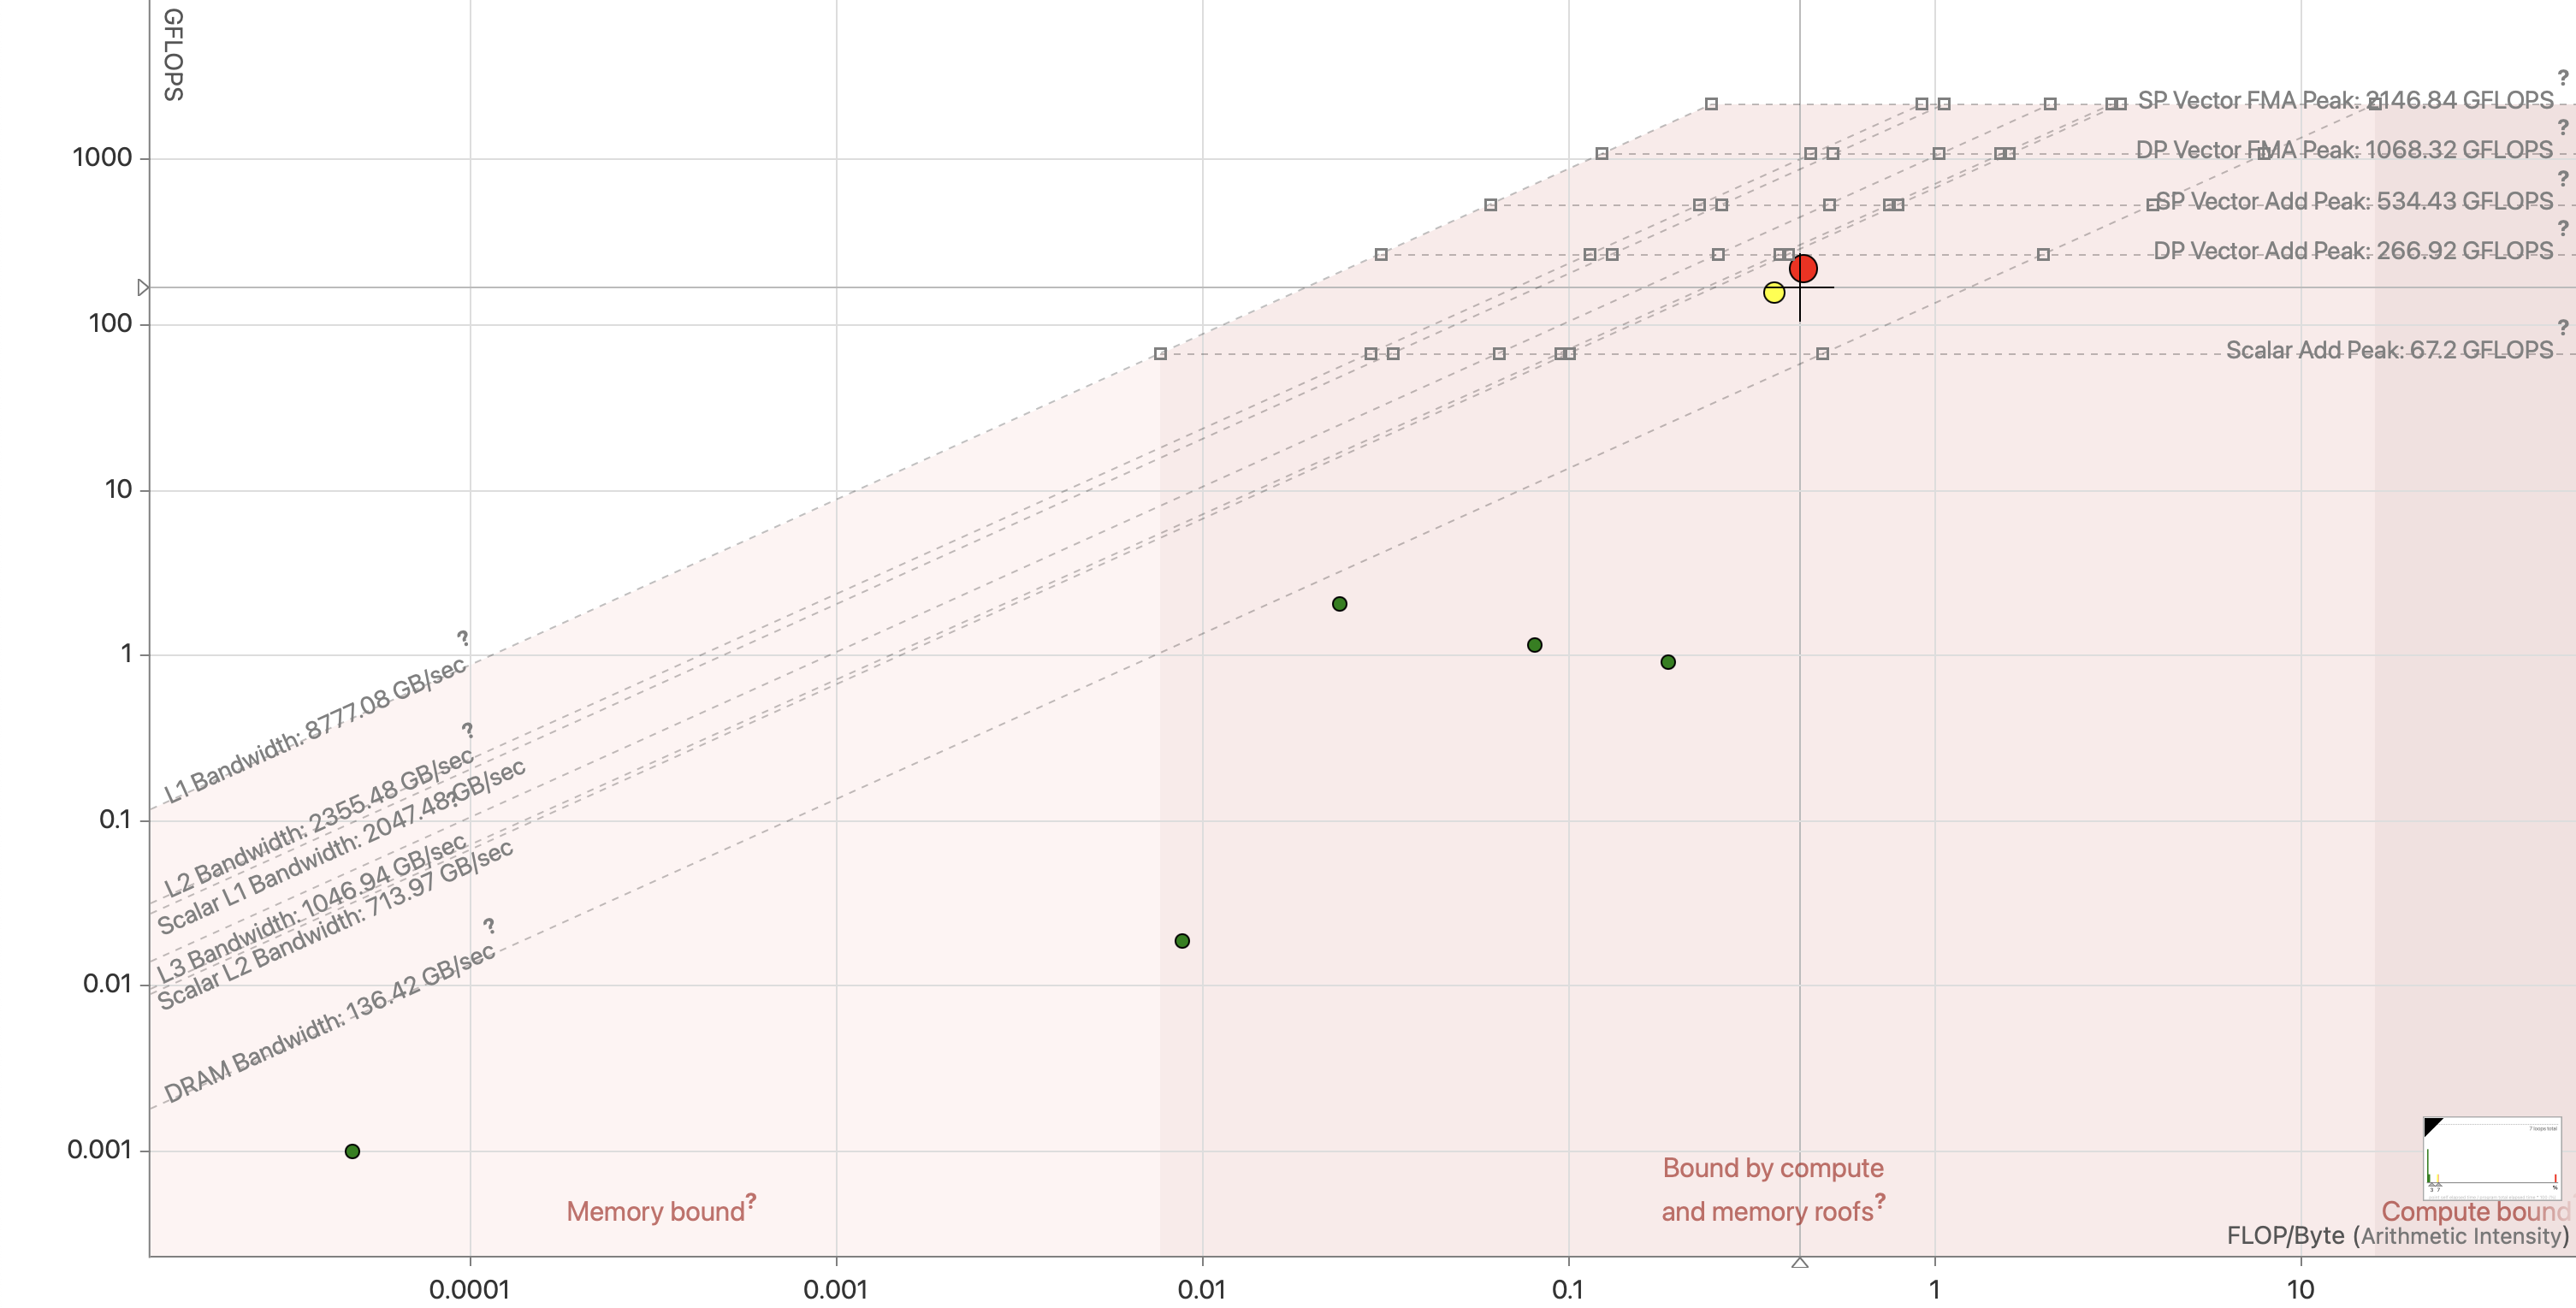
\includegraphics[width=\linewidth]{roofline_numa.png}
  \caption{Roofline model of my final implementation, run on the $1024\times1024$ test case}\label{fig:roofline_numa}
\end{figure}

Compared to my vectorized implementation, the arithmetic intensity was identical, whereas the performance increased by a factor of 16.60.
The increase in performance was primarily due to two main reasons.
Firstly, by running across multiple threads on multiple cores, the processor could compute sections of the grid in parallel.
Secondly, the parallel program did not have to interact with the DRAM, which had a lower bandwidth, as often.
When running on 28 cores, the parallel program had twice as much L3 cache, and 28 times more L1 and L2 cache than the serial program.
For example, in the \texttt{timestep} loop in the vectorized implementation, 5130.56 GB and 2306.03 GB of data were passed through the L1 cache and DRAM, respectively.
In the NUMA-aware implementation, 5777.32 GB and 1447.21 GB of data were passed through the L1 cache and DRAM, respectively. 

\section{LBM in Go}

Unlike C, Go is a language with concurrency built into its core design; consequently, one can implement parallelism effortlessly.
I sought to investigate whether one could achieve a similar level of performance using Go's core features.
I deemed this important since people frequently sacrifice small amounts of performance for a more straightforward implementation in real-world scenarios.

I produced an implementation of LBM in Go, \texttt{d2q9-bgk.go}, using an almost identical algorithm to that in \texttt{d2q9-bgk.c}.
The Go implementation was significantly slower in experiments, as evident in Table \ref{tab:go}.

\begin{table}[htbp]
  \begin{center}
  \caption{Execution times of \texttt{d2q9-bgk.go}, and speedup compared to the final \texttt{d2q9-bgk.c}}\label{tab:go}
  \begin{tabular}[t]{l | l l} 
      \hline\hline
      Grid Size&Time (s)&Speedup\\
      \hline
      $128 \times 128$&\texttt{ \space7.66}&\texttt{0.09}\\
      $128 \times 256$&\texttt{ 13.10}&\texttt{0.06}\\
      $256 \times 256$&\texttt{ 41.83}&\texttt{0.06}\\
      $1024 \times 1024$&\texttt{103.02}&\texttt{0.12}\\
      \hline
    \end{tabular}
  \end{center}
  \vspace{-1em}
\end{table}

The reasons for the comparatively poor performance included poor compiler optimisations and an unvectorized inner loop.
Methods exist to rectify these problems partially; however, they are directly contradictory to the desired simplicity of the experiment.
In conclusion, one cannot achieve a comparable level of performance from a more straightforward implementation using Go's core features.
% Compiling with GCCGO or GOLLVM may have produced a better-optimised executable; however, these required a complicated install#ation process, which was directly contradictory to the desired simplicity for the experiment.
% Vectorizing code in Go requires external libraries or assembly, which similarly conflicted with the desired simplicity.

\section{Conclusion}

In conclusion, the optimisations I utilised significantly improved the performance of \texttt{d2q9-bgk.c}.
Across the increasingly large test cases, my program achieved a speedup of 40.5x, 73.39x, 96.46x and 76.57x compared to the original implementation.
Vectorization and OpenMP multithreading provided the most significant improvements because both implemented some degree of parallelism: data level and task level, respectively.

\printbibliography

\end{document}